\section{问题二模型建立与求解}

\subsection{问题二分析}

问题二在每日零时承诺整天购电量，随后应对未知负载与光伏。计划量偏少时须支付五倍交易电价补足，偏多时仍按计划全额结算。这种非对称费用使采购量同时取决于预测值和误差分布。储能参与价格套利与误差补偿，当期误差还会改变后续可用电量，因此按完整轨迹评估。

本问采用“因果预测、整日残差场景、共同采购计划、实际状态反馈”的方案\cite{abunima2022,marino2018,grover2018}。母模型预先关闭额外CVaR及备用，即$\lambda=0$、$\rho_t=0$，场景数保留此前最多28条历史轨迹。预测器和执行器在一月验证中按实际账单选择，风险偏好与场景压缩只做后续对照。本问的候选筛选在开发期未取得节费收益，因此最终仍采用母模型；滚动问题的筛选选型另见第三问。

\subsection{问题二模型建立}

\begin{modelsummary}{问题二模型汇总}
\textbf{输入：}决策日前历史负载和光伏、已知电价及承接库存。\par
\textbf{决策：}144段共同购电计划、参考储能和场景紧急补购量。\par
\textbf{目标：}最小化全额计划费、期望五倍补购费与终端库存软罚之和。\par
\textbf{约束与输出：}28条整日残差场景满足供需不等式和储能界；贪心执行、日际SOC连续，输出购电计划、实际充放电、紧急量与结算账单。
\end{modelsummary}

\subsubsection{五倍补购费用为何导出80\%采购分位数}

先去掉储能和跨时段耦合，研究单时段基准。设$X$为实际净需求电量，$q\ge0$为计划采购，固定电价$p>0$，富余无残值，且$\mathbb E[X_+]<\infty$。概率和期望均以决策时已知信息为条件。期望费用为
\begin{equation}
 J_2(q)=pq+5p\,\mathbb E[(X-q)_+].
 \label{eq:mech_q2_cost}
\end{equation}
第一项是无论是否使用都要支付的计划费，第二项是计划不足时的补购费。记$F_X(x)=\Pr(X\le x)$、$F_X(x^-)=\Pr(X<x)$。$J_2$为凸函数，左右导数给出的次梯度为
\begin{equation}
 \partial J_2(q)=p[5F_X(q^-)-4,\ 5F_X(q)-4].
 \label{eq:mech_q2_subgradient}
\end{equation}
对于$q>0$的内点，最优解的充要条件是零属于其次梯度，即
\begin{equation}
 F_X(q^-)\le0.8\le F_X(q).
 \label{eq:mech_q2_quantile_condition}
\end{equation}
若分布在最优点连续，则$J_2'(q)=p-5p\Pr(X>q)=0$，化为$F_X(q)=0.8$；离散场景的概率跳跃由式\eqref{eq:mech_q2_quantile_condition}刻画。若最优点位于$q=0$边界，则右导数非负要求$F_X(0)\ge0.8$。以下分位数$F_X^{-1}(\alpha)=\inf\{x:F_X(x)\ge\alpha\}$表示，可选取
\begin{equation}
 q_2^\star=\max\{0,F_X^{-1}(0.8)\}.
 \label{eq:mech_q2_quantile}
\end{equation}
平坦分布区间可能导致多个最优解，上式给出其中一个。

80\%阈值源于计划价格与五倍补购价格的比例，说明偏高采购可由期望费用最小化产生。该解析式适用于无储能单时段；完整调度还须共同处理效率、功率、容量及跨时段库存价值。

\subsubsection{因果预测与决策导向选型}

问题二仅使用附件1电价和附件2历史负载、光伏。候选负载预测为前一周、最近2个或4个同星期日的同一时段均值，光伏预测为此前3、7或14个完整日的同一时段均值。以$X$表示负载，同星期预测写为
\begin{equation}
 \begin{cases}
 \displaystyle\widehat X_{D,t}=\frac{1}{|\mathcal W_D|}\sum_{j\in\mathcal W_D}X_{j,t},\\
 \mathcal W_D=\{D-7i:i=1,\ldots,K\}\cap\{1,\ldots,D-1\}.
 \end{cases}
 \label{eq:weekday_forecast}
\end{equation}
光伏移动均值改用此前$K$个完整日。历史不足时利用已有样本，没有相应星期日则退回近7日均值，首日采用附件1固定先验。其他问题的历史价格预测使用同一形式；各历史预测均按其当时可用数据生成。

借鉴按下游决策损失评价预测的思想\cite{elmachtoub2017spo}，本题固定场景和控制器，以实际结算费用比较预设预测器。

验证窗口为1月15--31日。所有候选从冻结旧版策略在1月15日的实际电量7081.8620 kWh开始，逐日因果运行，以计划费加紧急费选型。先固定28场景、零风险与零备用的内层LP，依次选择负载和光伏预测方法；随后固定预测器，比较贪心与内层LP。

% Generated by code/make_question_tables.py; do not edit values.
% Source: data/selection_v2.json; SHA256=f290084567f8b335dfbe7c042da7bf6863af20d3db001376f8bb5003dedd9aa7
\begin{table}[htbp]\centering\small
\caption{问题二预测器的一月实际费用验证}
\label{tab:q2-forecast-validation}
\begin{tabularx}{\linewidth}{LLLR}\toprule
比较步骤 & 负载预测 & 光伏预测 & 实际费用/元\\\midrule
负载比较 & 前一周 & 最近7日 & 933430.35\\
负载比较 & 同星期2日 & 最近7日 & 929216.46\\
负载比较 & 同星期4日 & 最近7日 & 930211.02\\
光伏比较 & 同星期2日 & 最近3日 & 928995.30\\
光伏比较 & 同星期2日 & 最近7日 & 929216.46\\
光伏比较 & 同星期2日 & 最近14日 & 932521.33\\
\bottomrule\end{tabularx}
\par\smallskip\parbox{\linewidth}{\footnotesize 此处固定内层LP及其余设置；相同配置复用同一次计算。随后单独比较执行器。费用不含终端目标项。}
\end{table}


由表\ref{tab:q2-forecast-validation}确定负载采用最近2个同星期日均值、光伏采用近3日均值。在这一预测组合下，贪心执行的一月费用917318.59元，内层LP为928995.30元，故主案选择贪心规则。两者验证末库存分别为7155.31和6000.00 kWh，与账单一并报告。

验证轨迹用于选型，已冻结旧版的一月实际运行提供共同前缀，各方案2月初态均为8875.1909 kWh。此后预测器类型、执行器及母模型设置固定，实际SOC逐日连续传递；采购候选筛选的适用问题与时点则由2--12月开发期比较确定。

\subsubsection{整日历史残差与场景构造}

在日期$D$的零时，取此前至多28个完整日组成$\mathcal H_D$。历史日$j$在时段$t$的净负荷残差为
\begin{equation}
 \begin{cases}
 \epsilon^n_{j,t}=
 \big[(L_{j,t}-R_{j,t})-(\widehat L_{j,t}-\widehat R_{j,t})\big]\Delta t,\\
 j<D.
 \end{cases}
 \label{eq:residual}
\end{equation}
每个历史日保留为完整144段轨迹，当前场景由
\begin{equation}
 \begin{cases}
 n_{t,s}=\widehat n_t+\epsilon^n_{j_s,t},\\
 \pi_s=1/|\mathcal H_D|,\\
 \displaystyle\sum_s\pi_s=1.
 \end{cases}
 \label{eq:q2_empirical_scenarios}
\end{equation}
给出，保留连续数小时共同偏高或偏低的误差。历史充足后排除采用固定先验的1月1日，主填报期均保留28条完整历史日轨迹。

场景缩减对照取最多12个代表日。对历史误差按整个残差块的总体标准差归一，计算轨迹间欧氏距离；先选总距离最小的代表，再逐次加入离已有代表最远的轨迹，随后交替分配样本与更新簇内medoid，至代表不变或达到8轮。每个代表仍是实际历史日，概率为所属簇频率；压缩后的经济效果通过闭环对照评价。

\subsubsection{受限两阶段采购模型}

日前第一阶段选择所有场景共享的计划$g_t$及参考$c_t,d_t,e_{t+1}$；补救阶段只允许紧急购电$h_{t,s}$随场景变化：
\begin{equation}
 \begin{cases}
 g_t+d_t+h_{t,s}-c_t\ge n_{t,s},\\
 h_{t,s}\ge0.
 \end{cases}
 \label{eq:scenario_balance}
\end{equation}
同一组参考充放电须在所有场景下配合相应紧急补购满足净需求。以
$Q_s=\sum_t5p_th_{t,s}$表示一条完整场景的紧急费用，主目标为
\begin{equation}
 \begin{cases}
 \displaystyle\min\left\{\sum_tp_tg_t+\sum_s\pi_sQ_s+
 \beta_T|e_{144}-6000|\right\},\\
 \beta_T=b_T\operatorname{median}_{t}p_t,\\
 b_T=1.
 \end{cases}
 \label{eq:q2_objective}
\end{equation}
第一项按零时计划全额计费，第二项为期望紧急费。第三项以偏离6000 kWh的软罚近似终端库存价值，绝对值通过正负偏差变量线性化。该罚项仅用于优化，实际账单按式\eqref{eq:q2_actual_bill}结算。容量、功率和状态方程沿用式\eqref{eq:soc}、\eqref{eq:limits}，初态为当日实际SOC，购电非负。

该受限两阶段模型在场景间共享储能参考；实际控制则利用逐时观测执行，形成独立的实际轨迹。参考与实际紧急费用的差异通过后续回放诊断，附件5填写实际动作。

\subsubsection{贪心执行器及状态连续性}

零时购电计划一经确定，本问全天令$a_t=g_t$。当期可观测的有效采购$a_t$、净需求$n_t$和储电量$e_t$决定实际动作。若$a_t\ge n_t$：
\begin{equation}
 \begin{cases}
 c_t^{\rm act}=\min\{a_t-n_t,U,(E_{\max}-e_t)/\eta_c\},\\
 d_t^{\rm act}=0,\\
 h_t=0,\\
 w_t=a_t-n_t-c_t^{\rm act}.
 \end{cases}
 \label{eq:execute_charge}
\end{equation}
若$a_t<n_t$：
\begin{equation}
 \begin{cases}
 d_t^{\rm act}=\min\{n_t-a_t,U,\eta_d(e_t-E_{\min})\},\\
 c_t^{\rm act}=0,\\
 w_t=0,\\
 h_t=n_t-a_t-d_t^{\rm act}.
 \end{cases}
 \label{eq:execute_discharge}
\end{equation}
然后按式\eqref{eq:soc}更新状态。常规富余用于充电，电池先补当期缺口，剩余缺口由紧急购电补足。充放电互斥、容量和功率界逐段满足。

日际满足$e_{D+1,0}=e_{D,144}$，库存连续传递。执行器只依赖当期合同、净需求与实测SOC；固定合同回放和内层LP对照用于检验这种规则与外层规划的差异。

经济主案保持零附加风险与零参考备用。风险、备用和场景压缩的定义及原母模型对照保留于\ref{app:optional_models}，用于检验保守程度的费用代价。

\subsection{问题二求解}

\subsubsection{逐日求解与评价口径}

每天零时先读取之前已完成的负载及光伏，更新冻结类型的预测器，再按式\eqref{eq:residual}构造28条场景；以当前实际SOC为初态求解外层LP，保存整日原计划和参考储能。随后每10分钟只揭示当前实际负载、光伏，按式\eqref{eq:execute_charge}或\eqref{eq:execute_discharge}执行，将本段充放电、紧急量及末态写入实际数组。当天结束后按
\begin{equation}
 C_D=\sum_{t=0}^{143}p_tg_{D,t}+\sum_{t=0}^{143}5p_th_{D,t}
 \label{eq:q2_actual_bill}
\end{equation}
结算实际费用，并把末态传至下一日。

正式评价范围为2025年2月1日至12月31日334天、每天144段。除核对费用可加性外，还检查实际电量平衡、SOC递推、充放电互斥、上下界、日际连续性以及全天$a_t=g_t$。指定日表、日汇总和附件5均从同一执行数组生成，原模板表头和列序保持不变。

表\ref{tab:q2-prediction-errors}用RMSE及MAE描述已选预测器在评价期的实际误差。
% Generated by code/make_question_tables.py; do not edit values.
% Source: data/selection_v2.json; SHA256=f290084567f8b335dfbe7c042da7bf6863af20d3db001376f8bb5003dedd9aa7
% Source: data/prepared_v2_q2.npz; SHA256=0322336272736ef1956aefa31f183bf42740abd1797e8d0d290fc61a700158fa
\begin{table}[htbp]\centering\small
\caption{问题二已选预测器的误差，单位为kW}
\label{tab:q2-prediction-errors}
\begin{tabularx}{\linewidth}{LRRRR}\toprule
变量 & 一月MAE & 一月RMSE & 评价期MAE & 评价期RMSE\\\midrule
负载 & 122.51 & 152.09 & 171.91 & 240.54\\
光伏 & 100.38 & 214.94 & 154.46 & 313.48\\
\bottomrule\end{tabularx}
\par\smallskip\parbox{\linewidth}{\footnotesize 一月指标取1月15--31日，评价期取2--12月。类型按一月结算费用选择，表中误差不用于重选。}
\end{table}


\subsubsection{总体结果与基础方案比较}

计划费用13507968.43元、紧急费用504839.24元，总费用14012807.66元；汇总均从原精度计算，分项舍入后可相差0.01元。评价期计划购电22047537.09 kWh，紧急购电85017.69 kWh，涉及113天、617个10分钟时段。共同期初库存8875.19 kWh、年末库存6240.32 kWh，与账单一并报告。

\begin{table}[htbp]\centering\small
\caption{问题2在相同预测与初态下的基础对照}
\label{tab:v2_baselines}
\begin{tabularx}{\linewidth}{LRRRR}\toprule
策略 & 总费/万元 & 紧急量/kWh & 日费CVaR95/元 & 末库存/kWh\\\midrule
无储能场景采购 & 1854.80 & 242340.86 & 80425.37 & 8875.19\\
点预测采购 & 1529.08 & 505585.75 & 100557.90 & 5845.40\\
场景期望费用（主案） & 1401.28 & 85017.69 & 70731.74 & 6240.32\\
\bottomrule\end{tabularx}
\par\smallskip\parbox{\linewidth}{\footnotesize 未启用候选筛选的母模型对照；各组沿用原实验配置，覆盖334天并连续推进状态。}
\end{table}


表\ref{tab:v2_baselines}三组采用相同预测和期初库存。点预测采购将单条预测曲线输入调度器，无储能场景采购禁用充放电，其他经济设置保持一致。点预测费用15290840.75元，主案节省1278033.08元，即8.36\%；相较无储能场景采购18548033.07元，主案费用降低24.45\%。结果体现了历史场景处理非对称补购代价与储能跨时段转移的作用，紧急购电则以五倍费用补足剩余负载。

图\ref{fig:q2-calendar-heatmap}按日期和物理时段展示紧急购电与时段末SOC，定位缺口及对应库存。零紧急量留浅灰，正值采用幂次色阶突出稀疏小额事件，色条标原始kWh；库存另用固定上下界色标。
\begin{figure}[htbp]\centering
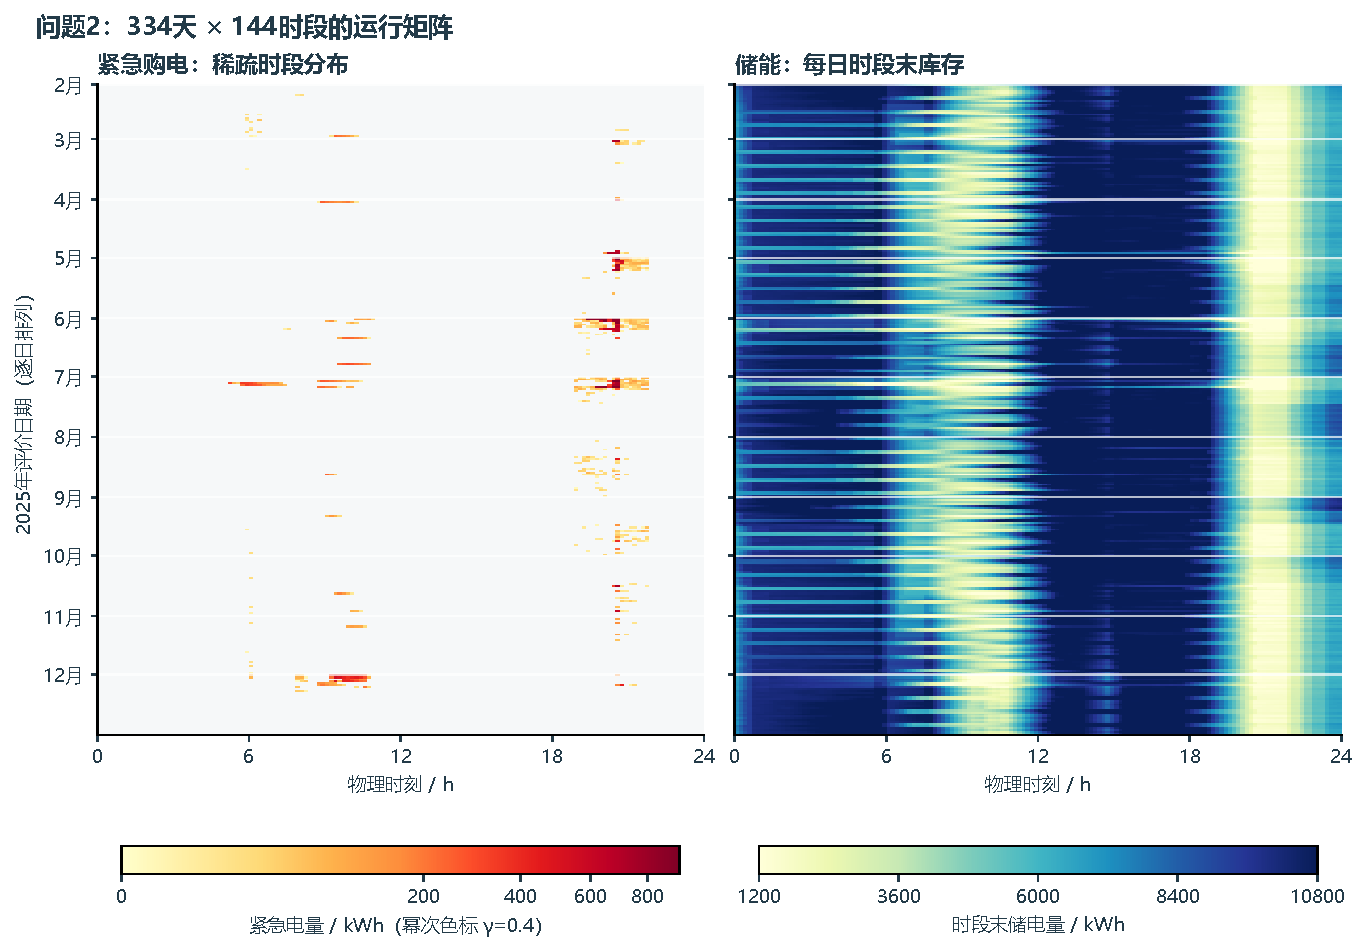
\includegraphics[width=0.97\linewidth]{figures/results/q2_calendar_heatmap.pdf}
\caption{问题二334个日期与144个物理时段的紧急量和时段末SOC；紧急量正值采用$\gamma=0.4$幂次色标，颜色数值仍以kWh标示}
\label{fig:q2-calendar-heatmap}
\end{figure}

基于执行规则回放的候选筛选在本问得到费用14035379.65元，比母模型增加22571.98元，即0.161\%，紧急量增至138015.18 kWh，因此本问保留母模型。滚动采购的筛选及时点比较见第三问。

\subsubsection{题目指定日期与完整策略填报}

\begin{table}[!htbp]\centering\small
\caption{问题二指定日期购电结果（电量：kWh）}
\label{tab:q2-purchase}
\setlength{\tabcolsep}{4pt}
\begin{tabularx}{\linewidth}{lRRRR}\toprule
物理时段 & 03-20 & 06-21 & 09-23 & 12-21\\\midrule
10:00--10:10 & 0.00 & 0.00 & 0.00 & 0.00\\
12:00--12:10 & 564.20 & 0.00 & 475.29 & 970.92\\
14:00--14:10 & 0.00 & 0.00 & 0.00 & 0.00\\
16:00--16:10 & 490.32 & 296.43 & 537.29 & 851.12\\
18:00--18:10 & 704.86 & 275.52 & 789.93 & 744.23\\
20:00--20:10 & 0.00 & 0.00 & 0.00 & 0.00\\
\midrule
全天常规量 & 67796.64 & 40036.30 & 69576.50 & 101008.53\\
全天实际费用/元 & 41219.41 & 23986.38 & 46384.26 & 65454.44\\
\bottomrule\end{tabularx}
\par\smallskip\parbox{\linewidth}{\footnotesize 日期均为2025年；购电量为零时计划量，紧急量单列。实际费用包含计划、调整及紧急三项账单。}
\end{table}

\begin{table}[!htbp]\centering\fontsize{10}{12}\selectfont
\caption{问题二指定日期储能结果（kWh）}
\label{tab:q2-battery}
\setlength{\tabcolsep}{4pt}
\begin{tabularx}{\linewidth}{lRRRR}\toprule
物理时段 & 03-20 & 06-21 & 09-23 & 12-21\\\midrule
00:00--04:00 & 3924.13 / 181.53 & 1394.50 / 465.11 & 4692.99 / 53.14 & 4499.79 / 40.16\\
04:00--08:00 & 1015.09 / 5240.21 & 460.19 / 4390.39 & 916.24 / 5893.48 & 762.27 / 1359.20\\
08:00--12:00 & 6123.03 / 2777.38 & 6534.90 / 0.00 & 5977.49 / 1896.62 & 5913.75 / 6490.57\\
12:00--16:00 & 3923.99 / 420.71 & 0.00 / 0.00 & 3708.39 / 625.98 & 5645.48 / 2130.65\\
16:00--20:00 & 268.54 / 5719.49 & 156.59 / 4882.20 & 151.78 / 5739.35 & 0.00 / 5526.27\\
20:00--24:00 & 5703.85 / 2960.43 & 6792.80 / 2485.90 & 5609.40 / 2640.89 & 5771.81 / 2842.53\\
\midrule
期初 / 期末库存 & 6705.54 / 6346.37 & 8644.37 / 8867.68 & 6006.02 / 6235.06 & 6794.81 / 6695.97\\
\bottomrule\end{tabularx}
\par\smallskip\parbox{\linewidth}{\footnotesize 六个时段行按“充电量 / 放电量”列示；末行为当日0时 / 24时库存。}
\end{table}

\begin{table}[!htbp]\centering\small
\caption{问题二指定日期紧急购电}
\label{tab:q2-emergency}
\setlength{\tabcolsep}{4pt}
\begin{tabularx}{\linewidth}{lLR}\toprule
日期 & 物理区间 & 紧急电量/kWh\\\midrule
03-20 & 无 & 0.00\\
06-21 & 无 & 0.00\\
09-23 & 20:20--20:40 & 388.40\\
 & 20:50--21:10 & 90.05\\
 & 21:20--21:50 & 34.20\\
12-21 & 无 & 0.00\\
\midrule
四日合计 &  & 512.64\\
\bottomrule\end{tabularx}
\par\smallskip\parbox{\linewidth}{\footnotesize 各日合计依次为0.00、0.00、512.64、0.00 kWh。}
\end{table}

\begin{table}[htbp]\centering\small
\caption{问题2指定日期计划、调整与费用分解}
\begin{tabularx}{\linewidth}{lRRRRR}\toprule
日期 & 计划量/kWh & 生效量/kWh & 计划费/元 & 调整费/元 & 紧急费/元\\\midrule
2025-03-20 & 67796.64 & 67796.64 & 41219.41 & 0.00 & 0.00\\
2025-06-21 & 40036.30 & 40036.30 & 23986.38 & 0.00 & 0.00\\
2025-09-23 & 69576.50 & 69576.50 & 43098.28 & 0.00 & 3285.98\\
2025-12-21 & 101008.53 & 101008.53 & 65454.44 & 0.00 & 0.00\\
\bottomrule\end{tabularx}\end{table}

四个指定日中，9月23日有三段紧急购电，合计512.64 kWh，其余三个指定日为零。其计划费43098.28元与紧急费3285.98元合计为全天实际费用46384.26元。相邻正值时段合并为同一紧急区间，间隔含零时保持分段。

表\ref{tab:q2-purchase}填写零时计划，紧急量单列于表\ref{tab:q2-emergency}。表\ref{tab:q2-battery}按四小时块累计实际充放电，每个10分钟段的动作保持互斥。完整计划保存在\texttt{result2.xlsx}，日费用由同源结果核对。
\FloatBarrier

